\documentclass[../body.tex]{subfiles}

\begin{document}
		\subsection{Оценки коэффициентов линейной регрессии}
		\subsubsection{Выборка без возмущений}
		\begin{itemize}
			\item Критерий наименьших квадратов: $$\hat{a}_{ls} \approx 1.86, \hat{b}_{ls} \approx 2.18$$
			\item Критерий наименьших квадратов: $$\hat{a}_{lm} \approx 1.9, \hat{b}_{lm} \approx 2.02$$
		\end{itemize}
	
		\begin{figure}[H]
		\centering
		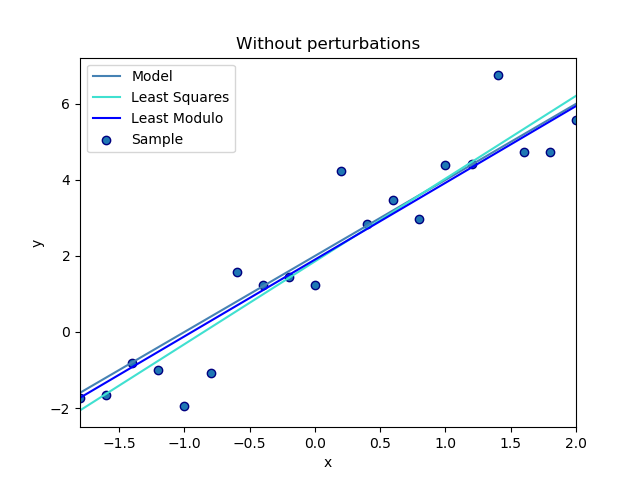
\includegraphics[width = 12cm, height = 9cm]{img/Without perturbations.png}
		\caption{Выборка без возмущений}
		\label{without}
	\end{figure}

	\subsubsection{Выборка с возмущениями}
	\begin{itemize}
		\item Критерий наименьших квадратов: $$\hat{a}_{ls} \approx 2.0, \hat{b}_{ls} \approx 0.77$$
		\item Критерий наименьших квадратов: $$\hat{a}_{lm} \approx 1.91, \hat{b}_{lm} \approx 1.95$$
	\end{itemize}
	
	\begin{figure}[H]
		\centering
		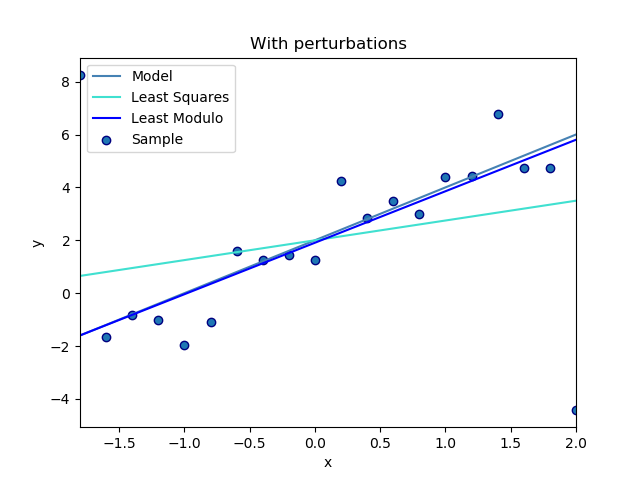
\includegraphics[width = 12cm, height = 9cm]{img/With perturbations.png}
		\caption{Выборка с возмущениями}
		\label{with}
	\end{figure}


\end{document}